\chapter{Numerics and Workflow}

    	 	\epigraph{On two occasions I have been asked, ``Pray, Mr. Babbage, if you put into the machine wrong figures, will the right answers come out?" ... I am not able rightly to apprehend the kind of confusion of ideas that could provoke such a question.}{Charles Babbage, Passages from the Life of a Philosopher}

Computational studies of the Navier-Stokes equations, especially as a dynamical system, are difficult for many reasons, but most important among them is the high degree of complexity inherent in the numerical tools required to maintain efficiency. As mentioned earlier, the two major approaches towards simulating Navier-Stokes are modeling, where some assumptions are made to reduce the difficult of simulation, and direct numerical simulation (DNS), where no assumptions beyond those used to derive Navier-Stokes and set up the boundary conditions are used. DNS is naturally more accurate (since the physicality of some modeling assumptions can be suspect), but in order to fully resolve the Navier-Stokes equations, it is significantly more computationally expensive than modeling. For this reason, I use the open source library {\tt Channelflow}\rf{Gibson2014}, which has been essential in making any headway in this thesis. {\tt Channelflow} is a spectral DNS library, with additional utilities to find, parametrically continue, and analyze \ecs, which I will lay out in some detail below.
\section{The Spectral Method}
\subsection{The Residual}

{\bf Spectral methods} are  part of a larger class of numerical methods known as {\bf weighted residual methods}. In this class of methods, functions are approximated by a truncated series expansion, with the restriction that a quantity related to the residual be zero (instead of the residual itself). The quantity used in spectral methods is the scalar product 
\begin{equation}\label{eq:scalarProduct}
\scprod{u}{v}{w} = \int{a}{b}{uvw}{dx},
\end{equation}
where  $u(x),v(x)$ are some functions on the interval $[a,b]$, and $w(x)$ is a weighting function. If we then imagine some platonic function (The function that is to be approximated) $u(x)$ that we attempt to approximate via a finite series expansion, so that
\begin{equation}\label{eq:seriesExpansion}
u_K(x) = \sum{k=0}{K}{\hat{u}_k \psi_k(x)},
\end{equation}
for some set of orthogonal basis functions $\psi_k(x)$, then the residual is given by
\begin{equation}
R_K = u(x)-u_K(x).
\end{equation} 
For a differential equation
\begin{equation}
Du = f,
\end{equation}
where $D$ is some arbitrary differential operator and $f(x)$ is some arbitrary source function, the residual is defined
\begin{equation}
R_K = Du_K - f.
\end{equation}
While it may seem logical to require $R_N = 0$, this is not possible in general for finite $N$, so we instead require that for a set of test functions $\phi_i(x)$ and weighting function $w^*$, the residual satisfies
\begin{equation}\label{eq:SpectralZero}
\scprod{R_N}{\phi_i(x)}{w^*} = R_N(x_i) = 0,
\end{equation}
for some set of $x_i$. If $\phi_i(x) = \delta(x-x_i)$ and $w^* = 1$, where
\begin{equation}
\delta(x-x') = 
\begin{cases}
0 &\text{if } x \neq x'\\
\infty &\text{if } x = x',
\end{cases}
\end{equation}
and
\begin{equation}
 \int{-\infty}{\infty}{\delta(x-x') = 1}{\textrm{d}x},
\end{equation}
 then we have the {\bf colocation method}, which forces the approximation to match the platonic function at a set of points. If $\phi_i(x) = \psi_i(x)$ and $w^* = w$, then we have the {\bf Galerkin method}, which forces the mean residual to be zero. 

\subsection{Basis Functions}

In the spectral method, trigonometric functions are chosen as the basis. The advantage of trigonometric functions over polynomials is the rapid convergence of the series coefficients -- the Fourier coefficients converge exponentially fast, so we can achieve extremely high accuracy with a lower number of modes\rf{Peyret2002}. However, spectral methods are inappropriate when the boundary geometry is highly complex, as is the case in the majority of industrial applications, where more general weighted residual methods are used. Since the plane Couette geometry is relatively simple, {\tt Channelflow} can make good use of the superior convergence rate of the spectral decomposition. {\tt Channelflow} uses Fourier series in the streamwise-spanwise directions, where the basis functions and spectral projection are given by 
\begin{align}
F_k(x) = \exp{ikx}\\
u_K(x) = \sum{k=-K}{K}\hat{u}_k\exp{ikx},
\end{align}
for both $x$ and $z$, and Chebyshev polynomials of the first kind in the wall-normal direction, where the basis functions and spectral projection are given by
\begin{align}
T_k(x) = \cos{k\arccos{x}}\\
u_N(x) = \sum{k=0}{(2k-1)/2}\hat{\mathfrak{u}}_kT_k(x).
\end{align}
\par The Fourier series expansion is particularly nice since the derivative $\partial_x F_k(x) = ikF_k(x)$ is especially easy to calculate, as are the Fourier coefficients by virtue of the Fast Fourier Transform, which is implemented in the Fastest Fourier Transform in the West (FFTW) library\rf{Frigo1998}.\\

For Chebyshev polynomials, the derivative is slightly more complicated, since 
\begin{equation}
\partial_x T_k(x) = 2k\sum{n=0}{(2k-1)/2}{\frac{1}{c_{k-1-2n}} T_{k-1-2n}(x)},
\end{equation}
where $c_k = 1$ if $k=1$ and $2$ if $k > 1$. Since the derivative of a single Chebyshev term becomes a sum of Chebyshev terms, the derivative of the Chebyshev representation of a function 
\begin{align}
\partial_x \sum{k=0}{K}\hat{\mathfrak{u}}_kT_k(x) &= \sum{k=0}{K}\hat{\mathfrak{u}}_k^{(1)}T_k(x),\\
\hat{\mathfrak{u}}_k^{(1)} &= \frac{2}{c_k}\sum{\substack{p = k+1\\(p+k) \mathrm{~odd}}}{K} p \hat{\mathfrak{u}}_p, \hspace{0.25cm} k \neq K,\\
\hat{u}^{(1)}_K &= 0.
\end{align}
As with the Fourier decomposition, however, Chebyshev coefficients can be calculated by a discrete cosine transform\rf{Halcrow2008}, which is a special case of the discrete Fourier transform, and is thus also computed efficiently by the FFTW. 

While Fourier expansions are the easiest to deal with, they are best used on periodic boundaries, since the imposition of aperiodic boundary conditions on a Fourier series expansion can lead to Gibbs oscillations that can make the simulation aphysical\rf{Peyret2002}. For this reason, the velocity field is expanded as a Fourier series in the plane, and as a Chebyshev polynomial in the wall-normal direction. Chebyshev polynomials can also easily satisfy the no-slip and no-penetration conditions \refeqs{eq:PCBC}{eq:NPBC}, and through the selection of the Gauss-Lobatto grid
\begin{equation}
x_{k} = \cos{\dfrac{k\pi}{N}},~k = 0,1,...K,
\end{equation}
naturally resolves the Navier-Stokes equations more accurately near the boundaries, where the increased accuracy is desirable. The velocity field is then represented as 
\begin{equation}
\Vector{u}_{KJL}(x,y,z) = \sum{k=-K}{K}{\hat{u}_k(x)\exp{ikx}}\sum{j=-J}{J}{\hat{u}_j(z)\exp{ijz}}\sum{l=0}{L}{\hat{\mathfrak{u}}_l(y)T_l(y)}.
\end{equation}

\subsection{Spatio-Temporal Discretization} 

Under the (Galerkin) spectral approximation 
\begin{equation}
\Vector{u}(x,y,z) = \Vector{U}_{KJL}(x,y,z),
\end{equation}
the partial differential equation
\begin{equation}
\pder{1}{\Vector{u}}{t} = f_T(\Vector{u}),
\end{equation}
becomes an extremely large set of ODEs
\begin{equation}
\der{1}{\Vector{U_{KJL}}}{t} = F_T(\Vector{U}_{KJL}), 
\end{equation}
where $f_T(\Vector{u})$ is the forward time evolution of the Navier-Stokes equation, and $F_T(\Vector{U}_{KJL})$ is its spectral approximation via \refeq{eq:SpectralZero}. The temporal ODE can be solved in any number of ways -- {\tt Channelflow} allows the user to choose from several implicit-explicit methods, where the implicit : Crank-Nicolson Forward Euler, Crank-Nicolson Adams-Bashforth, Spalart-Moser Runge-Kutta and Semi-implicit Backwards Differentiation of orders 1 to 4. The order 3 Semi-implicit Backwards Differentiation (SBDF3) was chosen by default, and no reason to change this was anticipated, since SBDF3 is known to have a relatively large time step and low error for large \ReN\rf{Ascher1995}.

\section{Newton-Krylov-Hookstep Method}

In order to find \ecs\, it is necessary to solve the equation
\begin{equation}\label{eq:NRResidual}
\Vector{u} - \sigma f_T(\Vector{u}) = \mathcal{R}_T(\Vector{u}) = 0,
\end{equation}
which is most easily tackled by root-finding algorithms. The root finding method used by {\tt Channelflow} is based on Newton's method with some additional refinements, which are discussed below. \\
\subsection{Newton's Method}
The principle behind Newton's method is as follows: Suppose  $f(x)$ is a smooth and differentiable function and that we have a `good' initial guess $x_0$ for one of its roots.\footnote{How good a guess needs to be is highly dependent on the problem. For this thesis, an initial condition that gave $\mathcal{R}_T(\Vector{u}) < 0.001$ was considered a sufficiently good guess.}  Then we can find a better guess for the root of $f$ by finding the root of the tangent line at $f(x_0)$, as shown in \refFig{fig:Newton}. Mathematically, 
\begin{align}
f(x_n) + f'(x_n)\paren{x_{n+1} - x_n} = 0,\label{eq:NRS1D}\\ 
x_{n+1} = x_n - \frac{f(x_n)}{f'(x_n)},\label{eq:NR1D}
\end{align}
where $x_n$ is the $n$-th guess for the root. In higher dimensions, \refeqs{eq:NRS1D}{eq:NR1D} are replaced by the matrix equations
\begin{align}
\Vector{f}(\Vector{x}_n) + \mathbb{J}_{f,\Vector{x_n}}(\Vector{x}_{n+1} - \Vector{x}_n) = 0,\label{eq:NRSND}\\
\Vector{x}_{n+1} = \Vector{x}_n - \mathbb{J}_{f,\Vector{x}_n}^{-1}\Vector{f}(\Vector{x}_n),
\end{align}
where $\mathbb{J}_{f,\Vector{x_n}}$ is the Jacobian of the Navier-Stokes equation at $\Vector{x}_n$.\\

\begin{figure}[h]
\includegraphics[width=\textwidth]{NRMethod}
\caption{A demonstration of Newton's method in 1D on a simple function with the root at $x_r \approx 8.98$. Starting at $x_0$ = 13, the first tangent (black) has a zero at $x_1 \approx 10.5$, the second tangent (red) has a zero at $x_2 \approx 9.4$, and the third tangent (green) has a zero at $x_3 \approx 8.99$. The method converges to within approximately $10^{-4}$ in just three steps.}\label{fig:Newton}
\end{figure}  

  \begin{figure}[h]
 \includegraphics[width=\textwidth]{NewtonOvershoot}
 \caption{If we assume the linear model remains valid for the entire step, we can sometimes be led astray. Because the function is linear only in the vicinity of the initial guess, the Newton step takes us very far away from the actual root we are trying to find, and will likely never converge.}\label{fig:NewtonOvershoot}
 \end{figure}
 
Newton's method is extremely fast and converges quadratically on the root\rf{Press2007}, but is not guaranteed to do so - a simple example is if the $n$-th guess is at (or very close to) a local minimum, in which case the second term of \refeq{eq:NR1D} will explode, taking us very far away from the initial, good guess, as in \refFig{fig:NewtonOvershoot}. Furthermore, in a system with around $10^5$ unknowns, inverting the Jacobian (or for that matter, finding the Jacobian) in \refeq{eq:NRSND} becomes very time consuming. To offset the inversion timing issue (we will deal with actually calculating the Jacobian later), we can trade off accuracy for speed by replacing  \refeq{eq:NRSND}  with a minimization problem
\begin{equation}\label{eq:minimizeNewt}
||\Vector{f}(\Vector{x}_n) + \mathbb{J}_{f,\Vector{x_n}}\Vector{dx}_n|| = r_n< \epsilon ||\Vector{f}(\Vector{x}_n)||,
\end{equation}
where $||\Vector{x}|| = \sqrt{\Vector{x} \cdot \Vector{x}}$ is the norm of $\Vector{x}$, $r_n$ is the residual at the $n$-th iteration, $\Vector{dx}_n = \Vector{x}_{n+1} - \Vector{x}_n$ and $\epsilon$ is some small parameter that controls how accurate we want the minimization to be\rf{Dembo1982}. Note that if $\epsilon = 0$, we recover \refeq{eq:NRSND}. Newton's method can be terminated either when successive steps fail to refine $\Vector{x}_n$ sufficiently, or when $f(\Vector{x})$ is sufficiently small.

\subsection{The Generalized Minimum Residual Method}

There are a vast quantity of residual minimization algorithms in existence, each typically optimized for a particular class of problem. {\tt Channelflow} uses the {\bf G}eneralized {\bf M}inimum {\bf RES}idual (GMRES) method, a Krylov subspace method developed in 1986 by Saad and Schultz\rf{Saad1986}. To illustrate the principle of GMRES, consider the least squares problem of finding the $\Vector{x} \in \mathbb{R}^n$ that minimizes
\begin{equation}\label{eq:AXB}
||\mathbb{A}\Vector{x} -\Vector{b}|| = r,
\end{equation}
where $\mathbb{A} \in \mathbb{R}^{n\times n}$ and $\Vector{b} \in \mathbb{R}^n$. The similarity of \refeq{eq:AXB} to \refeq{eq:minimizeNewt} makes the formulation of a solution to \refeq{eq:AXB} vital. 
\subsubsection{The Krylov Subspace}
Since \refeq{eq:AXB} is a model problem for \refeq{eq:minimizeNewt}, let $n \sim O(10^5)$. Since a search in such a huge space would be extremely time consuming, the GMRES method instead searches for a $\Vector{x}$ in a drastically lower dimensional {\bf Krylov subspace}. The $k$-th Krylov subspace for \refeq{eq:AXB} with a guess $\Vector{x}_0$ is defined
\begin{equation}\label{eq:krylov}
\mathcal{K}_k(\mathbb{A},\Vector{b}-\mathbb{A}\Vector{x_0}) = \mathrm{span}\paren{\Vector{b}-\mathbb{A}\Vector{x_0},\mathbb{A}\paren{\Vector{b}-\mathbb{A}\Vector{x_0}},\mathbb{A}^2\paren{\Vector{b}-\mathbb{A}\Vector{x_0}}...,\mathbb{A}^{k-1}\paren{\Vector{b}-\mathbb{A}\Vector{x_0}}},
 \end{equation}

 \subsubsection{The Arnoldi Iteration}
 
As mentioned earlier, both the calculation and inversion of the $\mathbb{A}$ are extremely difficult, precluding the use of \refeq{eq:krylov} to generate the Kyrlov subspace. The Krylov subspace is therfore generated via \refAlg{alg:Arnoldi}, known as the {\bf Arnoldi Iteration}. 
\begin{algorithm}\label{alg:Arnoldi}
Begin with $\Vector{q}_1 = \Vector{b} - \mathbb{A}\Vector{x}_0$. Then for the $k$-th Arnoldi iteration,
\begin{enumerate}
\item calculate $h_{ik} = \mathbb{A}\Vector{q}_{i} \cdot \Vector{q}_k,$ for $i = 1,2,...,k$,
\item generate $\Vector{p} = \mathbb{A}\Vector{q}_k - \sum{i=1}{k}{h_{ik}\Vector{q}_i},$ 
\item calculate $h_{k+1,k} = ||p||$,
\item and normalize $\Vector{q}_{k+1} = \frac{\Vector{p}}{h_{k+1,k}}$
\end{enumerate}
\end{algorithm}
Note something absolutely vital to the Arnoldi iteration - at {\bf no point} in the iteration is an explicit calculation of $\mathbf{A}$ necessary! Thus, we resolve the issue of calculating what will, in the case of {\tt Channelflow}, be the $10^5$ by $10^5$ Jacobian matrix.  Incidentally, the Arnoldi iteration is in general used to solve the eigenvalue problem for a matrix\footnote{That is, solving for the eigenvectors $\Vector{q}_k$ and eigenvalues $\lambda_k$ that satisfy $\mathbb{A}\Vector{q}_k = \lambda_k\Vector{q}_k$}, which will prove to be useful later. If we let $\mathbb{Q}_k = [ \Vector{q}_1| \Vector{q}_2 | ... |\Vector{q}_k ]$, and $[\mathbb{H}_k]_{ij} = h_{ij}$ if $h_{ij}$ exists, and $0$ otherwise, then 
\begin{equation}
\mathbb{H}_k = \mathbb{Q}_k^* \mathbb{A}\mathbb{Q},
\end{equation}
and 
\begin{equation}\label{eq:Qiter}
\mathbb{A}\mathbb{Q}_k = \mathbb{Q}_{k+1}\mathbb{\tilde{H}}_k,
\end{equation}
where $\mathbb{\tilde{H}}_k$ is $\mathbb{H}_k$ with an additional row $[0,0,0...,h_{k+1,k}]$. Following the derivation in \rf{Ipsen1998}, if $\Vector{z} \in \mathcal{K}_k(\mathbb{A},{\Vector{b}-\mathbb{A}\Vector{x_0}})$, 
\begin{equation}
\Vector{z} = \mathbb{Q}_k \Vector{y},
\end{equation}
for some $\Vector{y}$. Then 
\begin{align}
\begin{split}
\mathbb{A}\Vector{z} &= \mathbb{A}\mathbb{Q}_{k}\Vector{y},\\
				&= \mathbb{Q}_{k+1}\mathbb{\tilde{H}}_{k}\Vector{y},
\end{split}
\end{align}
so by restricting our guess to the Krylov subspace, \refeq{eq:AXB} can be written as 
\begin{equation}\label{eq:shutUpMatt}
|| \mathbb{Q}_{k+1}\tilde{\mathbb{H}}_k \Vector{y} - \paren{\Vector{b}-\mathbb{A}\Vector{x_0}} || = r.
\end{equation}
Since multiplication by a unitary matrix does not affect the norm, \refeq{eq:shutUpMatt} becomes
\begin{equation}\label{eq:UNIMATRIX}
|| \mathbb{Q}^*_{k+1}\mathbb{Q}_{k+1}\tilde{\mathbb{H}}_k \Vector{y} - \mathbb{Q}^*_{k+1}\paren{\Vector{b}-\mathbb{A}\Vector{x_0}}|| = r,
\end{equation}
\begin{equation}
||\tilde{\mathbb{H}}_k \Vector{y} - \mathbb{Q}^*_{k+1}\paren{\Vector{b}-\mathbb{A}\Vector{x_0}}|| = r. 
\end{equation}

The second term of the norm is a vector of the form 
\begin{equation}\label{eq:QS}
\mathbb{Q}^*_{k+1}\paren{\Vector{b}-\mathbb{A}\Vector{x_0}} = \begin{pmatrix} \Vector{q}_1^*\paren{\Vector{b}-\mathbb{A}\Vector{x_0}} \\ \Vector{q}_2^*\paren{\Vector{b}-\mathbb{A}\Vector{x_0}} \\  \vdots \\ \Vector{q}_{k+1}^*\paren{\Vector{b}-\mathbb{A}\Vector{x_0}}  \end{pmatrix},
\end{equation}
but since, from the definition of the Krylov subspace, $\mathbb{Q}_1 = \textrm{span}\paren{\Vector{b}-\mathbb{A}\Vector{x_0}}$ = $[\Vector{q}_1]$, 
\begin{equation}
\Vector{q}_1 = \dfrac{\Vector{b}-\mathbb{A}\Vector{x_0}}{||\Vector{b}-\mathbb{A}\Vector{x_0}||}.
\end{equation}
Since the Arnoldi iteration naturally produces an orthonormal set of $\Vector{q}_i$, \refeq{eq:QS} simplifies to 
\begin{equation}
 \mathbb{Q}^*_{k+1}\paren{\Vector{b}-\mathbb{A}\Vector{x_0}} = \begin{pmatrix} ||\Vector{b}-\mathbb{A}\Vector{x_0}|| \\ 0 \\  \vdots \\ 0 \end{pmatrix} =  ||\Vector{b}-\mathbb{A}\Vector{x_0}|| \begin{pmatrix}1 \\ 0 \\  \vdots \\ 0 \end{pmatrix} =  ||\Vector{b}-\mathbb{A}\Vector{x_0}|| \Vector{e}_1.
\end{equation}
Substituting this into \refeq{eq:UNIMATRIX} provides the final residual problem
\begin{equation}\label{eq:GMRESMIN}
|| {||\Vector{b} - \mathbb{A}\Vector{x}_0||}\Vector{e}_1 - \mathbb{\tilde{H}}_k \Vector{y} || = r,
\end{equation}
that is solved by \refAlg{alg:GMRES}.
  \begin{algorithm}\label{alg:GMRES}
   Begin with
 \begin{align*}
 \Vector{c} &= \Vector{b} - \mathbb{A}\Vector{x}_0,\\
  \Vector{q}_1 &= \frac{\Vector{c}}{||c||}, \\
  \mathbb{Q}_1 &= [\Vector{q}_1],\\
  \mathcal{K}_1(\mathbb{A},\Vector{c}) &= \mathrm{span}(\Vector{q}_1).
  \end{align*}
  Then the $k$-th GMRES iteration is given by  
  \begin{enumerate}
  \item generating $\Vector{q}_{k+1}$, $\mathbb{Q}_{k+1}$ and $\mathbb{\tilde{H}}_k$ via the Arnoldi iteration,
  \item finding the $\Vector{y}_{k+1}$ that minimizes \refeq{eq:GMRESMIN},
  \item and computing $\Vector{x}_{k+1} = \mathbb{Q}_{k+1}\Vector{y}_{k+1}$.
  \end{enumerate}
  \end{algorithm}

 The second step of \refAlg{alg:GMRES} may seem nonsensical - why have we put this much effort into getting an equation similar to \refeq{eq:AXB}? The key lies in realizing that the minimization problem in  \refAlg{alg:GMRES} has a dimension of $k$, whereas \refeq{eq:AXB} has a dimension on the order of $10^5$. Since the matrix inversion problem scales as dimension to the third power, this reduction is extremely powerful -- especially since GMRES converges quickly -- in this thesis, GMRES rarely took more than 20 iterations to converge. The minimization step in  \refAlg{alg:GMRES} can be solved via a QR decomposition, with a time complexity of $O(n)$\rf{Trefethen1997}.  
 
 \subsection{The Hookstep}
 
 While Newton's method is incredibly powerful, it needs to be provided a sufficiently good guess to stand a chance of converging to a solution. However, in practice, we are limited in our ability to provide good guesses with our computing resources, since we are searching for the proverbial needle in a $10^5$ dimensional haystack. As a consequence, even our best guesses may be less than ideal for a pure Newton method -- for example, the linear model used in deriving Newton's method may not be valid for the Newton step $\Vector{dx}_N$, as shown in \refFig{fig:NewtonOvershoot}. 

 
 If this is the case, switching to a constrained {\bf hookstep} can force the algorithm to take artificially smaller steps, until the linear model becomes locally accurate. In {\tt Channelflow}, the equation of constraint for the hookstep $\Vector{dx}_H$ is 
 \begin{equation}\label{eq:HSEOC}
 ||\Vector{dx}_H|| \leq \delta,
 \end{equation}
 where $\delta$ is known as the {\bf trust region} of the local linear model -- that is, the region around the guess where the function remains approximately linear.  The hookstep is further restricted to lie in the $k$-th Krylov subspace, so that 
 \begin{equation}\label{eq:HSKRYPROJ}
 \Vector{dx}_H = \mathbb{Q}_{k}\Vector{s},
 \end{equation} 
 where $\Vector{s}$ is now the $k$-dimensional step we need to take. As with the Newton step, the hookstep is determined using GMRES. Unlike the Newton step, the minimization stage of \refAlg{alg:GMRES} is not computed via the QR decomposition\rf{Gibson2014}. Instead, we substitute \eqref{eq:Qiter} and \eqref{eq:HSKRYPROJ} into \eqref{eq:AXB}, giving the residual which we wish to minimize with respect to $\Vector{s}$,
 \begin{equation}\label{eq:HSRes}
 ||\mathbb{Q}^{T}_{k+1}\Vector{b}-\mathbb{\tilde{H}}_k\Vector{s}|| = r.
 \end{equation}
 Applying the singular value decomposition\footnote{The singular value decomposition is a method by which a matrix $\mathbb{A} \in \mathbb{R}^{n\times m}$ is factorized into the product $\mathbb{U}\mathbb{D}\mathbb{V}^T$, where $\mathbb{U} \in \mathbb{R}^{n\times n}$ and $\mathbb{V} \in \mathbb{R}^{m\times m}$ are unitary matricies, and $\mathbb{D} \in \mathbb{R}^{n\times m}$ is a diagonal matrix. }, $\mathbb{\tilde{H}}_k = \mathbb{U}\mathbb{D}\mathbb{V}^T$ transforms \eqref{eq:HSRes} intro
 \begin{equation}
 || \Vector{\hat{b}}-\mathbb{D}\Vector{\hat{s}} || = r,
 \end{equation}
 where $\Vector{\hat{s}} = \mathbb{V}^T\Vector{s}$, $\Vector{\hat{b}} = \mathbb{U}^T\mathbb{Q}^T_{k+1}\Vector{b}$. Using Lagrange multipliers, the minimization problem in \refAlg{alg:GMRES} yields the solution\rf{Gibson2014}
 \begin{equation}
 {\hat{s}}_i = \frac{{\hat{b}}_i {D}_{ii}}{{D}_{ii}^2 + \mu},
 \end{equation}
 where $\mu$ minimizes 
 \begin{equation}
 ||\Vector{\hat{s}}(\mu)||^2 - \delta^2 = \mathfrak{r},
 \end{equation}
 which can be trivially solved by a 1D Newton method. 
 
 \section{Recurrence Diagrams}
 
 While the augmentation of the Newton-Krylov method by the hookstep makes it more resilient against poor guesses, the Newton-Krylov-Hookstep (NKH) method remains extremely sensitive to initial conditions. As a result, a method to generate decent guesses to kickstart the NKH solver is vital. One way to do this is to try to find some underlying pattern in a trajectory that could hint at the presence of \ecs. For example, we could view the trajectory in the dissipation and energy input plane, as in\rf{Viswanath2007}, which has proven successful in the past. Generalizing this method, we can consider the {\bf recurrence diagram} of the trajectory, which can be generated via \refAlg{alg:rec}. \\
 
  \begin{algorithm}\label{alg:rec}
  \textcolor{white}{haha}
 \begin{enumerate}
 \item Begin with an initial condition. This can be chosen by randomly generating a field, or making a slight random perturbation off a known \ecs.
 \item Integrate this initial condition forward in time using SBDF3 to obtain a trajectory 
 \item Calculate some metric of the trajectory that provides insight into its dynamical structure
 \item Extract some number of good guesses from this metric, and pass them along to the NKH solver.
 \end{enumerate}
 \end{algorithm} 
In particular, calculating the metric  
\begin{equation}\label{eq:recurrenceEQ}
 \mathfrak{R}(t,T) = ||\Vector{u}(t+T) - \Vector{u}(t)||,
 \end{equation}
where $\mathfrak{R}(t,T)$ measures the distance of the field at time $t+T$ from the field at time $t$. When using this metric, the recurrence diagram naturally becomes a method by which the spatio-temporal separation of successive flow states in a trajectory can be visually and numerically analyzed, since small values of $\mathfrak{R}$ indicate points in the $(t,T)$ plane where the spatio-temporal separation of the field is also small. Interpretation of a recurrence diagram is not an exact science - for example, a naive search for the minimum of \refFig{fig:recurrenceMinimum} would yield all the points for which $T=0$. Experience has shown that long, horizontal streaks of low values correspond to the shadowing of a periodic orbit, and tend to be excellent sources of good guesses for the NKH solver. \\
 
\begin{figure}[h]
\includegraphics[width=\textwidth]{RecPlot}
\caption{A recurrence plot which was used to find one of the new periodic orbits (P60) presented in this thesis. At each point, the value of  $\mathfrak{R}(t,T) = ||\Vector{u}(t+T) - \Vector{u}(t)||$ is plotted. Light colorations correspond to low values, and vice versa. Notice the long, thin streak of low values from $t = 200$ to $t = 450$  for $T \approx 60$. A guess sourced from this band was the initial guess that led to the discovery of P60.}\label{fig:recurrenceMinimum}
\end{figure}
 \refeq{eq:recurrenceEQ} is only useful for \ecs\ with no relative velocity, and thus can only be applied when neither spanwise nor streamwise symmetry is broken. To deal with the case when streamwise or spanwise symmetry is broken, we modified \refeq{eq:recurrenceEQ} to allow for the possibility of relative solutions, by changing the problem to finding small values of 
 \begin{equation}\label{eq:4DrecurrenceEQ}
 \mathfrak{R}(t,T,l_x,l_z) = ||\tau(l_x,l_z)\Vector{u}(t+T) - \Vector{u}(t)||.
  \end{equation}
 This is now a 3 or 4 dimensional minimization problem, since we now need to find low values of $\mathfrak{R}$ in the recurrence domain $[t_0,t']\times [0,T_{\textrm{max}}] \times [l_{x,~\textrm{min}},l_{x,~\textrm{max}}] \times [l_{z,~\textrm{min}},l_{z,~\textrm{max}}]$. The most obvious consequence of the increase in the domain dimension is that the time complexity of calculating $\mathfrak{R}$ increases from $O(n^2)$ to up to $O(n^4)$. A more fundamental issue, however, is that the visual approach to analyzing recurrence diagrams  now appears unusable, since visualizing a 4D domain is not practical. We sidestep the issue by developing and using \refAlg{alg:recBroke}. \refAlg{alg:recBroke}, however, does nothing to offset the significant increase in calculations needed to fully calculate the recurrence diagram. However, a glance at \refFig{fig:recurrenceMinimum} shows that a large part of the diagram contains no patterns at all, and is functionally useless. For this reason, when working with symmetry broken trajectories, the initial recurrence diagram is computed at a significantly lower resolution than it would have been for a trajectory in the fully symmetric space. When features are identified in the low resolution recurrence diagram, we can construct a higher resolution diagram around the features that are worthy of further consideration. The has the effect of reducing the time required to find good guesses from multiple days to a single day. 

\begin{algorithm}\label{alg:recBroke}
For a trajectory $\Vector{u}(t)$ with a recurrence domain   $[t_0,t']\times [0,T_{\textrm{max}}] \times [l_{x,~\textrm{min}},l_{x,~\textrm{max}}] \times [l_{z,~\textrm{min}},l_{z,~\textrm{max}}]$, 
\begin{enumerate}
\item for a $(t,T) \in [t_0,t']\times [0,T_{\textrm{max}}]$, 
\item find $\mathfrak{R}(t,T,l_x,l_z)$ for each $(l_x,l_z) \in  [l_{x,~\textrm{min}},l_{x,~\textrm{max}}] \times [l_{z,~\textrm{min}},l_{z,~\textrm{max}}]$ and 
\item save only the smallest $\mathfrak{R}$ and the minimizing $(l_x,l_z)$ found this way,   
\end{enumerate}
 for each $(t,T) \in [t_0,t']\times [0,T_{\textrm{max}}]$.
\end{algorithm}

\begin{figure}[h!]
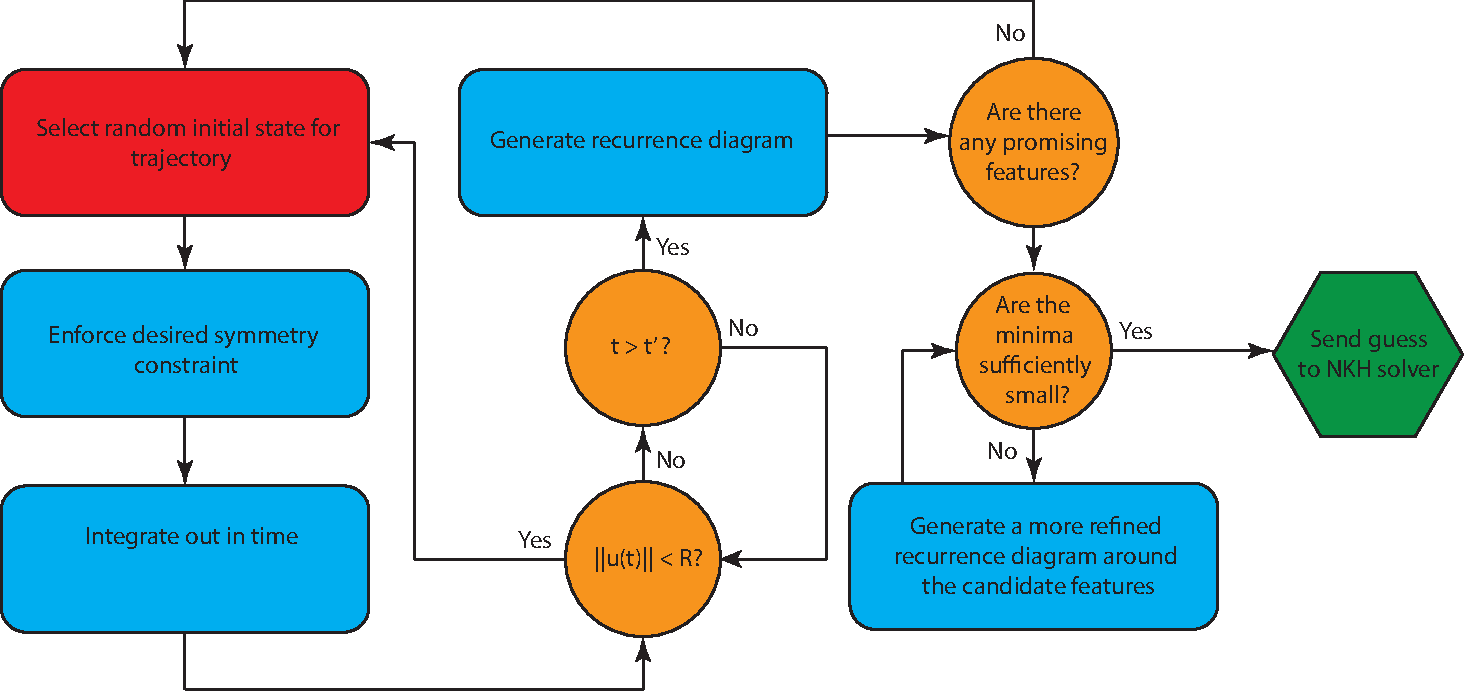
\includegraphics[width=\textwidth]{FlowChart}
\caption{A flow chart that lays out the procedure used to find \ecs. We begin by selecting a random initial state for the trajectory. This initial state can either be found by generating a truly random state, or by applying a small, random perturbation to a known \ecs. The desired symmetry constraints are then enforced, and the trajectory is integrated from $t = 0$ to $t=t'$. After every time step, if the state's norm has dropped below some threshold $R$, we assume that the trajectory has relaminarized, and find a new initial condition to work with. Once the integration is over, we generate the recurrence diagram according to \refeq{eq:recurrenceEQ}, for some $T_{\textrm{max}}$, and attempt to find any patterns we would associate with \ecs. If no patterns are found, we find another initial state and repeat the process. If there are some candidate patterns, we calculate the minimum $\mathfrak{R}$ of that feature. If it is below some threshold, we accept it as a potential solution, and pass it to the NKH solver. If $\mathfrak{R}$ is not low enough, it is likely not a sufficiently good guess to cause the NKH solver to converge in a reasonable time, so we zoom in on the pattern and calculate a refined recurrence graph, until either the minimum value of the pattern is low enough, or it becomes apparent that the pattern is unlikely to produce a meaningful initial guess}\label{fig:FlowChart} 
\end{figure}
 \clearpage
 \section{Parametric Continuation} 
 
 If we have a solution to \refeq{eq:NRResidual} for some control parameters, such as \ReN\ or the cell size, we may wish to see how these solutions vary with these control parameters. For example, if we know that a solution $S$  exists for $\ReN = 400$, we might want to know how this solution differs from the solution , $S'$ at $\ReN = 200$, assuming that $S'$ exists. The solution may, for example vary as in \refFig{fig:bifurcations},  One of the most efficient ways to find these solutions is via \refAlg{alg:parCont}, known as {\bf parametric continuation}.
 \begin{algorithm}\label{alg:parCont}
 If we have a solution $S_{\mu_0}$ with a control parameter $\mu_0$,  and a solution finding method $\mathfrak{S}(S,\mu)$, then $S_{\mu_k}$ can be found by
 \begin{enumerate}
 \item choosing a $\mu_{i+1} = \mu_{i} + \mathrm{d}\mu$ such that the residual $\mathfrak{S}(S_{\mu_{i}},\mu_{i+1})$ is small,
 \item and then using $S_{\mu_i}$ as a guess for $\mathfrak{S}$ to find $S_{\mu_{i+1}}$,
 \end{enumerate}
 for $i = 1,2,..,k-1$.
 \end{algorithm}
\par
At this point, the underlying numerical framework has been laid bare to the point that it is at the very least, a slightly gray box. Applying the methods of the previous chapters took a great deal of trial and error\footnote{More of the latter}, but has nevertheless proven successful. In the following chapter, I will present four new periodic orbits for \pCf\, and discuss their properties.   
 \begin{figure}[h]
 \includegraphics[width=\textwidth]{BifurcationDiagram}
 \caption{A schematic of a 1D bifurcation, that shows the variation of a solution $x^*$ as a function of a control parameter $r$. While the control parameter $r < 2$, there is only one, stable solution, on the left. At a critical value $r = 2$, however, a new solution emerges at $x^* = 1$ in a {\bf saddle-node bifurcation}. When $2 < r < 4$, the saddle-node splits into two, producing a stable solution (solid) on the right, and an unstable solution (dashed) on the left. As $r$ approaches 4, the original stable solution and the new unstable solution approach each other until at $r=$, they annihilate in another saddle node bifurcation, leaving only the new stable solution. In higher dimensions, bifurcations can be incredibly complex, but we can nevertheless observe bifurcations of this form. }\label{fig:bifurcations}
 \end{figure}
 
 